\documentclass[a4paper,11pt]{article}

\usepackage[top=0.5in, bottom=1in, left=0.8in, right=0.8in, headsep=0.in, centering]{geometry}
\usepackage[utf8]{inputenc}
\usepackage{amsmath}
\usepackage{amsfonts}
\usepackage{amssymb}
\usepackage{graphicx}
\usepackage{amsthm}
\usepackage{caption} 
\usepackage{array}
\usepackage{amsmath}
\usepackage{bookmark}
\usepackage{enumitem}

\newcommand\innerprd[1][.5]{\mathbin{\vcenter{\hbox{\scalebox{#1}{$\bullet$}}}}}
\newcommand\ntsb[3]{\makebox[#1cm][c]{$\overset{#2}{#3}$}}
\newtheorem{theorem}{Theorem}[section]
\newtheorem{lemma}[theorem]{Lemma}
\newtheorem{proposition}[theorem]{Proposition}
\newtheorem{corollary}[theorem]{Corollary}
\newtheorem*{conjecture}{Conjecture}
\theoremstyle{definition}
\newtheorem{definition}[theorem]{Definition}
\newtheorem{example}[theorem]{Example}
\newtheorem{remark}[theorem]{Remark}
\newtheorem{assumption}[theorem]{Assumption}
\newtheorem{problem}[theorem]{Problem}
\newtheorem{property}[theorem]{Property}

\def\Xint#1{\mathchoice
{\XXint\displaystyle\textstyle{#1}}%
{\XXint\textstyle\scriptstyle{#1}}%
{\XXint\scriptstyle\scriptscriptstyle{#1}}%
{\XXint\scriptscriptstyle\scriptscriptstyle{#1}}%
\!\int}
\def\XXint#1#2#3{{\setbox0=\hbox{$#1{#2#3}{\int}$}
\vcenter{\hbox{$#2#3$}}\kern-.5\wd0}}
\def\ddashint{\Xint=}
\def\dashint{\Xint-}


%%%%%%%%%%%%%%%%%%%%%%%%%%%%%%%%%%%%%%%%%%%%%%%%%%%%%%%%%%%%%%%%%%%%%%%%%%%%%%%%%%%%%%%%

\title{
Seed document}

\author{
    Kiyuob Jung\thanks{Department of Mathematics, Kyungpook National University, Daegu, 41566, Republic of Korea, E-mail:~kyjung2357@gmail.com}}

\begin{document}
\date{}
\maketitle

%%%%%%%%%%%%%%%%%%%%%%%%%%%%%%%%%%%%%%%%%%%%%%%%%%%%%%%%%%%%%%%%%%%%%%%%%%%%%%%%%%%%%%%%

\section{Section Title}

In this section, we provide some examples for LaTeX.

\subsection{Code Example}

\noindent I prefer to use `'$\innerprd$' for inner products since is bigger than `'$\cdot$'.

\noindent Here, I provide some integrations:
\begin{equation*} 
    \dashint, \quad \ddashint, \quad \Xint\circlearrowright, \quad \Xint\circlearrowleft,\quad  \Xint\subset, \quad \Xint\infty.
\end{equation*}

\noindent Use the new command `nstb' to note on symbols, for example, $\ntsb{0.5}{?}{=}$, $\ntsb{0.5}{(1.1)}{\leq}$. 

\noindent As for citation, 
Also, you can refer to \cite{2010_Evans} in the bibtex file.

\subsection{Picture}

Here, one can insert a picture.
Note that the picture file should be included in the same folder including this tex file.

\begin{figure}[h]
    \centering
    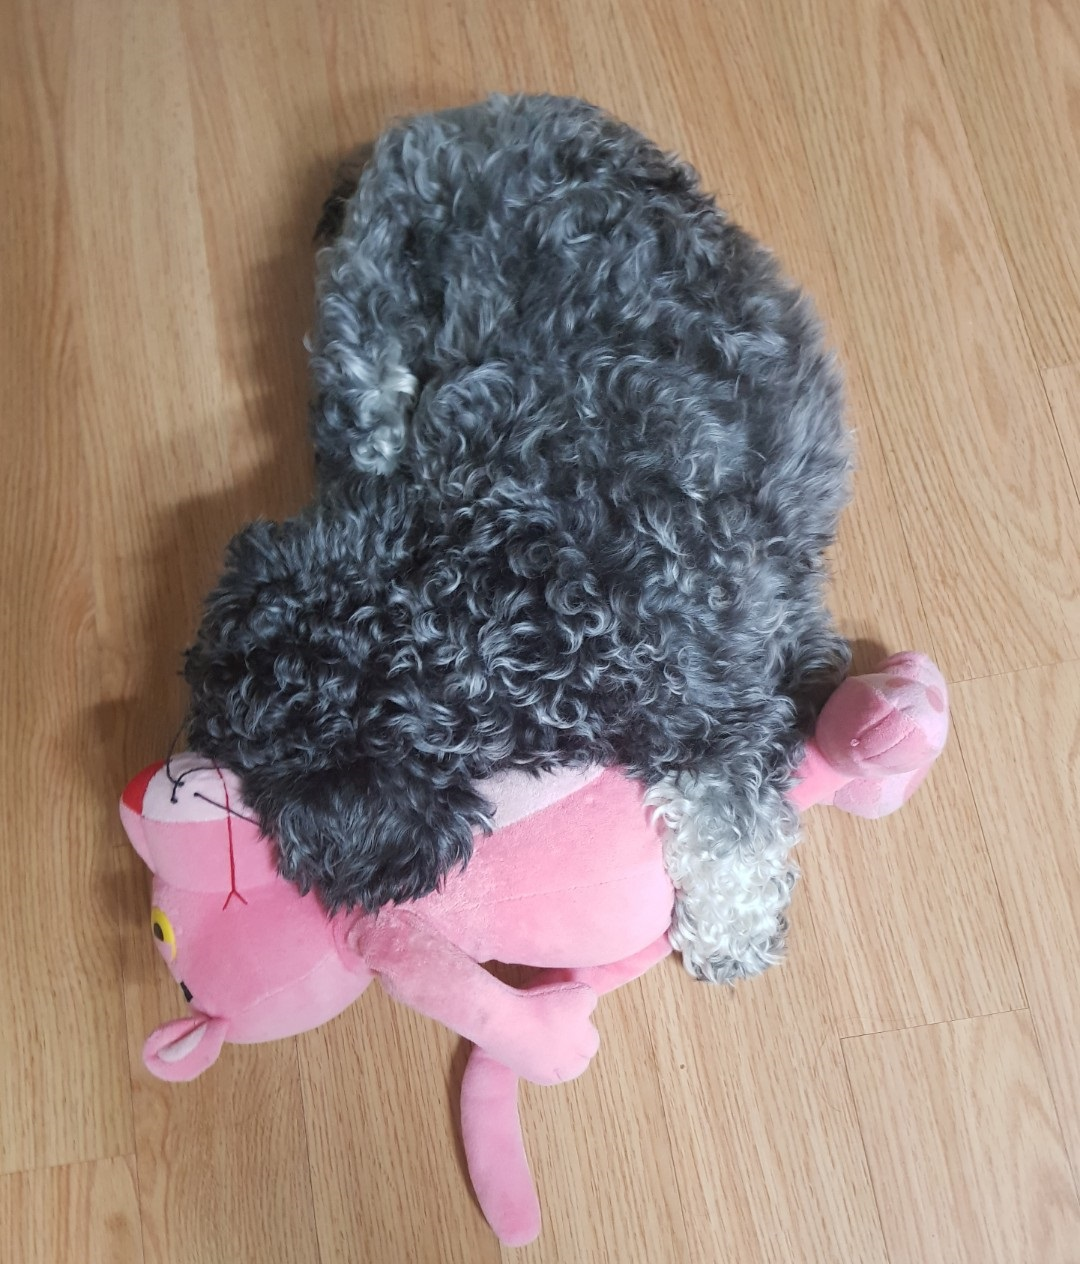
\includegraphics[width=0.2\textwidth]{write the name of the picture}
    \caption{write the caption}
    \label{fig:my label}
\end{figure}
\noindent Write Figure \ref{fig:my label} to refer the above picture.

\subsection{Statement Example}


\begin{theorem}
    Write a statement.
\end{theorem}

\begin{proof}
    SKIP.
\end{proof}





\bibliographystyle{abbrv}
\bibliography{bibliography}{}

\end{document}



